% Keine komplizierten Relationships
% Folie 46: Relationship - Diverses
% Folie 47: Diverses
% Folien 84 - 87: Lazy Loading (aber Folie 80 relevant > Wissen um was es sich handelt)
% Folien 96-105: Kapitel "OR-MappingAdvanced"

\section{Entity Framework}

\begin{multicols*}{2}
Entity Framework Core /EF Core ist ein O/R Mapping Framework und verbindet Objekt-Orientiertes (Domain Model) mit
Relationalem (Relational Model). 
Man unterscheidet zwischen verschiedenen Varianten wie die Entitätsklassen/Datenbanken erstellt werden könnnen:
\includegraphics*[width=\columnwidth]{ef}

\subsection{Database Context (DbContext)}
Unsere NameContext Klasse leitet von DbContext ab und darauf wird spezifiziert was die
Datenbank machen / wissen muss.
\begin{lstlisting}
public class ShopContext : DbContext { /* ... */ }
\end{lstlisting}
\begin{itemize}
    \item Wichtigster Teil des Entity Frameworks
    \item Interagiert mit der Datenbank
    \item Hat verschiedene Funktionen zu Design-Time und Run-Time
\end{itemize}
\fat{Design-Time:}
\begin{itemize}
    \item Model definieren (OR Mapping)
    \item Konfiguration
    \item Database Migrations
\end{itemize}
\fat{Run-Time:}
\begin{itemize}
    \item Connections verwalten
    \item CRUD Operationen ausführen
    \item Change Tracking
    \item Caching
    \item Transaction Management
    \item uvm.
\end{itemize}
\subsubsection{Lifecycle}
DbContext-Instanzen sollten nicht
\begin{itemize}
    \item zu lange leben
        \begin{itemize}
            \item Limitierte Anzahl Connections im Client Connection Pool
            \item Change-Tracking wird über die Zeit ineffizient
        \end{itemize}
    \item geshared werden
        \begin{itemize}
            \item Ist nicht thread-safe
            \item Exception kann Instanz unbrauchbar machen
        \end{itemize}
\end{itemize}
\fat{Empfehlungen:} 
\begin{itemize}
    \item In einem using-Statement verwenden
    \item Web Applikationen: Instanz pro Request
    \item GUI: Instanz pro Formular
    \item Generell: Instanz pro Unit of Work
\end{itemize}

\subsubsection{Fluent API Configuration}
Konfiguration von vielen Klassen / Entity Types im gleichen Context führt zu unübersichtlichem Code.
Es kann für jede Entity eine Config Klasse erstellt werden, welche innerhalb des Contexts dann aufgerufen werden kann.
\begin{itemize}
    \item Config Klasse implementiert IEntityTypeConfiguration<T> Interface
    \item Configure Methode wird überschrieben mit der Fluent API Konfiguration des Entity Types
    \item modelBuilder.ApplyConfiguration führt für jede Config die Methode Configure aus.
\end{itemize}
\begin{lstlisting}
internal class CategoryTypeConfig
    : IEntityTypeConfiguration<Category>
{
    public void Configure(
        EntityTypeBuilder<Category> builder)
    {
        builder
            .Property(p => p.Timestamp) 
            .IsRowVersion();
    } 
}

public class ShopContext : DbContext 
{
    protected override void OnModelCreating(
        ModelBuilder modelBuilder)
    {
        modelBuilder.ApplyConfiguration(
            new CategoryTypeConfig() );
    }
}
\end{lstlisting}

\subsubsection{LINQ to Entities}
Entity Framework führt keine Queries aus sondern generiert sie nur. Datenbank führt sie dann aus.\\ 
Nicht alle .NET-Expressions können auf Datenbanksyntax übersetzt werden.
Vorallem solche mit eigenen Klassen und Funktionen sind problematisch.
\begin{lstlisting}
//Funktionierendes Beispiel
await context.Categories.SingleAsync(c => c.Name.ToLower() == "tablets")
//Fehlerhaftes Beispiel
await context.Categories.SingleAsync(c => MyHelper.DoSomethingWithIt(c.Name) == "tablets")
\end{lstlisting}
\fat{LINQ Beispiel:}
\begin{lstlisting}
//DbContext instanzieren
using (ShopContext context = new()) {
    //Abfrage mit LINQ (direkt)
    Category category = await context 
        .Categories
        .SingleAsync(c => c.Id == 1);
    
    //Daten ändern / speichern
    category.Name = \$"{category.Name} / Changed";
    await context.SaveChangesAsync();
    
    //Abfrage mit LINQ (deferred)
    var categories = context.Categories;
    foreach (Category c in categories)
    {
        Console.WriteLine(c.Name);
    }
} //DbContext schliessen
//Cache invalidieren / DB-Verbindung zurück in Connection Pool
\end{lstlisting}
\fat{Generierter SQL Output:}
\begin{itemize}
    \item Je nach Formulierung unterschiedlich
    \item Manchmal optimal, manchmal weniger
    \item Kann von Version zu Version ändern
\end{itemize}
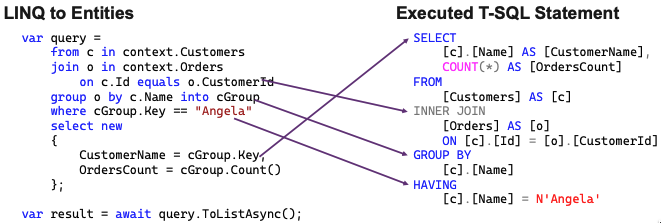
\includegraphics[width=\columnwidth]{linqsql}

\subsection{DbContext: CUD Operationen}
\begin{itemize}
    \item DbContext agiert nach dem Unit of Work (UoW) pattern
    \item Objekt wird beim Laden aus der Datenbank automatisch der UoW registriert
    \item Änderungen werden aufgezeichnet. Beim Speichern werden alle Änderungen in einer einzigen Transaktion geschrieben.
\end{itemize}
\subsubsection{Insert}
\begin{lstlisting}
using ShopContext context = new();

Category cat = new() { Name = "Notebooks" };

// Add to Context (3 alternatives)
// - Use .Add(...) to apply to whole graph (Category which has already assigned products with orders) 
// - Use .State when only for this entity (ignoring the objects laying behind the category)
context.Add(cat); 
context.Categories.Add(cat); 
context.Entry(cat).State = EntityState.Added;

//Save - SQL is executed here
await context.SaveChangesAsync();

// Check Primary Key
// Category.Id was created in DB after saving changes
int id = cat.Id; 
\end{lstlisting}
\subsubsection{Update}
\begin{lstlisting}
using ShopContext context = new();

Category cat = await context
    .Categories
    .FirstAsync();

// Change-Tracker marks this object as changed
cat.Name = "Changed";

// Save - SQL is executed here
await context.SaveChangesAsync();
\end{lstlisting}
\subsubsection{Delete}
\begin{lstlisting}
using ShopContext context = new();

Category cat = await context
    .Categories
    .FirstAsync(c => c.Name == "Notebooks");

// Remove (3 alternatives)
// - Use .Remove(...) to apply to whole graph 
// - Use .State when only for this entity 
context.Remove(cat); 
context.Categories.Remove(cat); 
context.Entry(cat).State = EntityState.Deleted;

// Save - SQL is executed here
await context.SaveChangesAsync();
\end{lstlisting}

\subsection{DbContext: CUD Operationen von Assoziationen}
\begin{itemize}
    \item Durch Anpassung von Navigation Properties
    \begin{lstlisting}
//Bestehender Customer wird durch neuen ersetzt
order.Customer = customer;
    \end{lstlisting}
    \item Hinzufügen / Entfernen von Elementen in Collection Navigation Properties
    \begin{lstlisting}
//Bestehender Customer wird gelöscht, dann neuer hinzugefügt
customer1.Orders.Add(order);
customer2.Orders.Remove(order);
    \end{lstlisting}
    \item Setzen des Foreign Keys (einzige Variante, welche keine weiteren Datenbankzugriffe benötigt)
    \begin{lstlisting}
//Foreign Key wird auf neuen Customer umgemappt
order.CustomerId = 1;
    \end{lstlisting}
\end{itemize}
\subsubsection{Insert Object Graph}
\begin{lstlisting}
using ShopContext context = new();
Customer cust = new()
{
    Name = "Anna",
    Orders = new List<Order> {
        new() { /* ... */ },
        new() { /* ... */ },
    } 
};

// Add whole object graph to Context
context.Add(cust);
    
// Save - SQL is executed here
await context.SaveChangesAsync();
\end{lstlisting}
\subsubsection{Insert Related Entity}
\begin{lstlisting}
using ShopContext context = new();

Customer cust = await context
    .Customers
    //Stellt sicher dass alle orders geladen werden
    .Include(c => c.Orders)
    .FirstAsync(); 

cust.Orders.Add(new Order());
    
// Save - SQL is executed here
await context.SaveChangesAsync();
\end{lstlisting}

\subsubsection{Change Relationship}
\fat{Beispiel 1: Zwei DB-Zugriffe}\\
Change via Navigation Property.
\begin{lstlisting}
using ShopContext context = new();

Order order = await context
    .Orders
    .FirstAsync();

// Replace old customer with customer Angela
order.Customer = await context
    .Customers
    .FirstAsync(c => c.Name == "Angela");

// Save - SQL is executed here
await context.SaveChangesAsync();
\end{lstlisting}
\fat{Beispiel 2: Ein DB Zugriff}\\
Change via Foreign Key, wenn dieser schon bekannt.
\begin{lstlisting}
using ShopContext context = new();

Order order = await context
    .Orders
    .FirstAsync();

// Change
order.CustomerId = 2;
    
// Save - SQL is executed here
await context.SaveChangesAsync();
\end{lstlisting}

\subsection{DbContext: Object Graph / Ladestrategien}
\fat{Definition: } ''Set of individual, but related objects, that together form a logical whole unit''
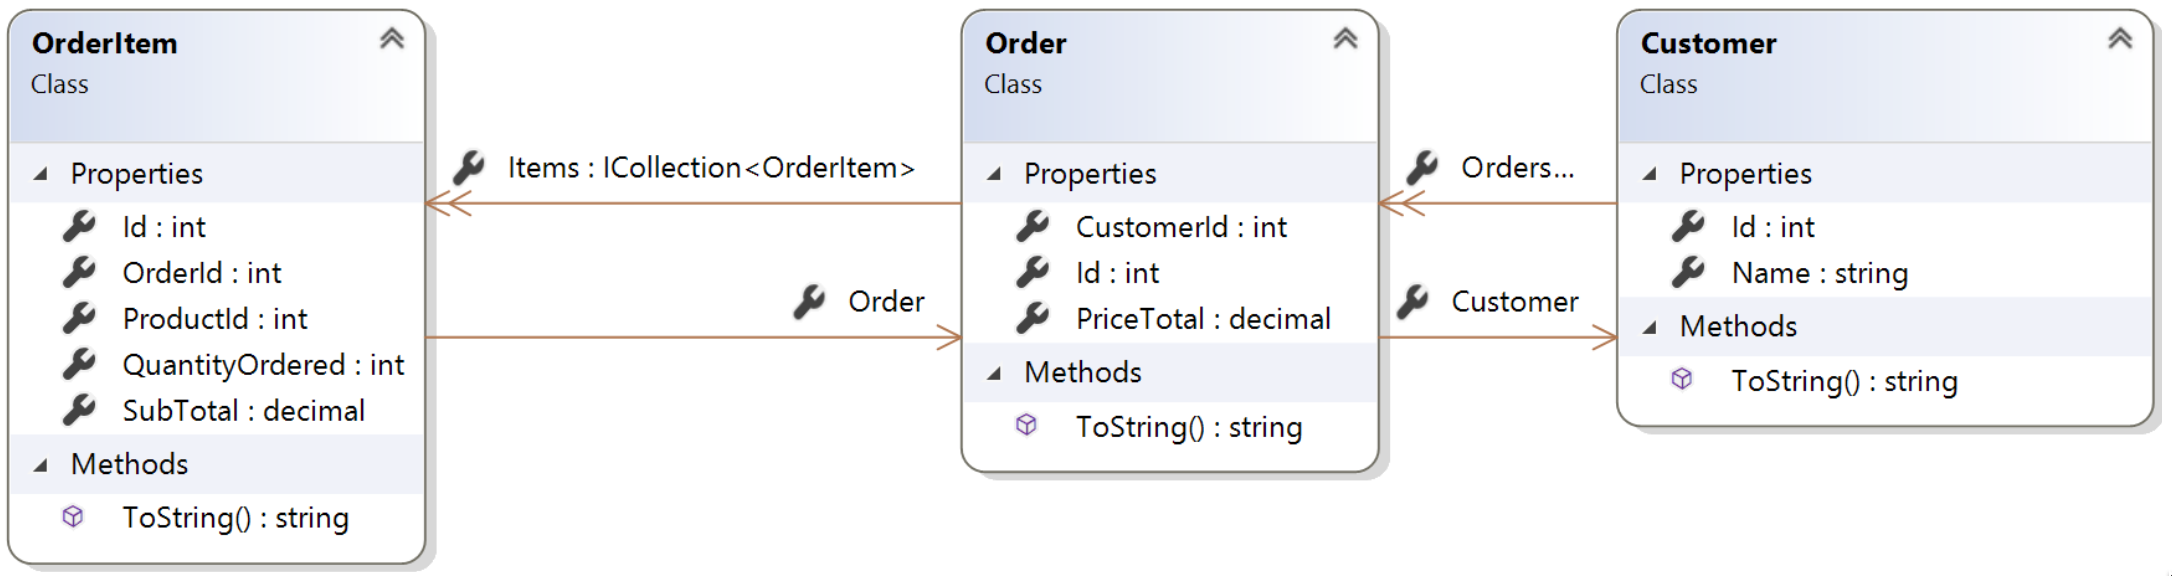
\includegraphics[width=\columnwidth]{objgraph}
\fat{Was wird bei diesem Graphen geladen?} Zu dieser Frage gibt es
verschiedene mögliche Strategien.
Bei diese Abfrage besteht keine Möglichkeit auf Customer oder Items zuzugreifen, da nur order geladen wurde.
\begin{lstlisting}
Order order = await context 
    .Orders
    .FirstAsync();

var customer = order
    .Customer; // customer is "null"
var items = order
    .Items; // items is "null"
\end{lstlisting}
\subsubsection{Eager Loading (Default)}
\begin{itemize}
    \item Assoziationen werden per se nicht geladen
    \item Include()-Statement für einzelne Assoziationen
    \item Passiert in der gleichen Abfrage per JOIN
\end{itemize}
\begin{lstlisting}
Order order = await context 
    .Orders
    .Include(o => o.Customer) //Eager Loading
    .Include(o => o.Items)
    //Zusätzliches Laden der Product Tabelle hinter Items
        .ThenInclude(oi => oi.Product)
    .FirstAsync();
var customer = order
    .Customer; // customer is not "null"
var items = order
    .Items; // items is not "null"
\end{lstlisting}
\subsubsection{Explicit Loading}
\begin{itemize}
    \item Assoziationen werden per se nicht geladen
    \item Assoziationen werden explizit nachgeladen
    \item Collections werden komplett geladen
    \item Passiert in separater Abfrage $\rightarrow$ mehrere SQL Statements   
\end{itemize}
\begin{lstlisting}
Order order = await context 
    .Orders
    .FirstAsync();

await context
    .Entry(order) //Holt Change Tracker Eintrag
    .Reference(o => o.Customer)  //Lade ein Customer
    .LoadAsync();

await context
    .Entry(order)
    .Collection(o => o.Items) //Lade viele Items
    .Query() //Start Filter
    .Where(oi => oi.QuantityOrdered > 1) //FilterKriterium
    .LoadAsync();

var customer = order
    .Customer; // customer is not "null"
var items = order
    .Items; // items is not "null"
\end{lstlisting}
\subsubsection{Lazy Loading}
\begin{itemize}
    \item Assoziationen werden per se nicht geladen
    \item Assoziationen werden bei Zugriff auf Property automatisch nachgeladen
    \item Collections werden komplett geladen / Filtern aber möglich
    \item Passiert in separater Abfrage $\rightarrow$ mehrere SQL Statements 
    \item Kann gefährlich sein, da z.B. bei Zugriff auf Property die Connection im DbContext schon weg sein könnte
\end{itemize}

\subsection{DbContext: Change Tracking}
\begin{itemize}
    \item Registriert alle Ändungen an getrackten Entities
    \item Aktualisiert den Entity State
    \item Agiert komplett offline: Keine Live-Checks auf Datenbank
\end{itemize}
\subsubsection{Entity States}
\begin{itemize}
    \item Under Change Tracking
    \begin{itemize}
        \item Unchanged
        \item Added
        \item Modified
        \item Deleted
    \end{itemize}
    \item Not Tracked
    \begin{itemize}
        \item Detached
    \end{itemize}
\end{itemize}
\subsubsection{Methoden für State Tracking}
.Add / .Remove / etc. berücksichtigen ganzen Objekt-Graphen\\
.Entry(...).State nur die jeweilige Entity
\begin{itemize}
    \item Add(): State Added
    \item Remove(): State Deleted
    \item Update(): State Updated
    \item Unchanged(): State Unchanged
\end{itemize}
\subsubsection{State Transition Example}
\begin{lstlisting}
// New Record -> EntityState.Detached
Category cat = new() { Name = "Laptops" }; 

context.Add(cat); //EntityState.Added
await context.SaveChangesAsync(); //EntityState.Unchanged

cat.Name = "Notebooks"; //EntityState.Modified
await context.SaveChangesAsync(); //EntityState.Unchanged

context.Remove(cat); //EntityState.Deleted
await context.SaveChangesAsync(); //EntityState.Unchanged

// Load from Database (tracked)
Category loaded1 = await context //EntityState.Unchanged
    .Categories
    .FirstAsync(c => Name == "Tablets" ); 

// Load from Database (untracked) 
Category loaded2 = await context //EntityState.Detached
    .Categories
    .AsNoTracking()
    .FirstAsync(c => Name == "Smart Phones" );
\end{lstlisting}

\subsection{OR-Mapping (Platform unabhängig)}
Ein OR-Mapper (Mapping) stellt die Verbindung zwischen Datenbank (Storage Entity) und Klassen (Entity Type) her.
\begin{itemize}
    \item \fat{Providers:} Diverse relationale SQL Providers. Andere Provider über NuGet verfügbar
    \item \fat{Entity:} Normale .NET Klassen. Strukturierter Datensatz mit einem Key. Gruppiert in Entity Sets
    \item \fat{Mapping:} Mapping der Klassen auf das darunter liegende Speichermodell:
    \begin{itemize}
        \item By Convention
        \item By Attributes
        \item By Fluent API
    \end{itemize}
    Zuordnung von:
    \begin{itemize}
        \item Entity Type zu Storage Entity
        \item Property zu Column
        \item Entity Key zu Primary Key
        \item Foreign Key zu Relationship
    \end{itemize}
    \item \fat{Storage Entity:} Relationales Modell. Abhängig von gewähltem Provider
\end{itemize}
\includegraphics*[width=\columnwidth]{or}
\subsubsection{Include / Exclude von Properties}
Klasse Category soll auf die Datenbank abgebildet werden.
\fat{Convention:}
\begin{lstlisting}
public class ShopContext : DbContext 
{
    //Context mitteilen dass Category abgebildet wird
    public DbSet<Category> Categories { get; set; }  
}

public class Category
{
    public int Id { get; set; }
    public string Name { get; set; }
    //Klasse Produkt wird implizit auch abgebildet
    public ICollection<Product> Products { get; set; } 
    public ICollection<Metadata> Metadata { get; set; }
}
public class Product { /* ... */ } 
public class AuditEntry { /* ... */ }
public class Metadata { /* ... */ }
\end{lstlisting}
\fat{Data Annotations:}
\begin{lstlisting}
[NotMapped] //Exclude
public class Metadata { /* ... */ }  
\end{lstlisting}
\fat{Fluent API:}
\begin{lstlisting}
public class ShopContext : DbContext {
    protected override void OnModelCreating(ModelBuilder modelBuilder)
    {
        //Include
        modelBuilder.Entity<AuditEntry>(); 
        //Exclude
        modelBuilder.Ignore<Metadata>();
    } 
}
\end{lstlisting}

\subsubsection{Include / Exclude von Properties}
\fat{Convention:}
Alle public Properties mit Getter/Setter
\nfat{Data Annotations:}
\begin{lstlisting}
public class Category {
    public int Id { get; set; }
    public string Name { get; set; }
    [NotMapped]
    public DateTime LoadedFromDatabase { get; set; }
}
\end{lstlisting}
\fat{Fluent API:}
\begin{lstlisting}
protected override void OnModelCreating(ModelBuilder modelBuilder)
{
    modelBuilder.Entity<Category>()
        .Property(b => b.Name);
    modelBuilder.Entity<Category>()
        .Ignore(b => b.LoadedFromDatabase);
}
\end{lstlisting}
\subsubsection{Keys}
\fat{Convention:}
Property mit dem Namen ''[Entity]Id''
\begin{itemize}
    \item Beispiel 1: Category.Id
    \item Beispiel 2: Category.CategoryId
\end{itemize}
\fat{Data Annotations:}
\begin{lstlisting}
public class Category
{
    [Key]
    public int Id { get; set; } 
    public string Name { get; set; }
}
\end{lstlisting}
\fat{Fluent API:}
\begin{lstlisting}
protected override void OnModelCreating(ModelBuilder modelBuilder)
{
    modelBuilder.Entity<Category>()
        .HasKey(e => e.Id);
}
\end{lstlisting}
\subsubsection{Required / Optional}
\fat{Convention:}
\begin{itemize}
    \item Value Types werden NOT NULL (int)
    \item Nullable Value Types werden NULL (int?)
    \item Reference Types werden NULL
\end{itemize}
\fat{Data Annotations:}
\begin{lstlisting}
public class Category
{
    public int Id { get; set; } 
    [Required]
    public string Name { get; set; } 
    public bool? IsActive { get; set; }
}
\end{lstlisting}
\fat{Fluent API:}
\begin{lstlisting}
protected override void OnModelCreating(ModelBuilder modelBuilder)
{
    modelBuilder.Entity<Category>()
        .Property(e => e.Name)
        .IsRequired();
}
\end{lstlisting}
\subsubsection{Maximum Length}
\fat{Convention:}
\begin{itemize}
    \item Keine Restriktion / z.B. NVARCHAR(MAX)
    \item 450 Zeichen bei Keys
\end{itemize}
\fat{Data Annotations:}
\begin{lstlisting}
public class Category
{
    public int Id { get; set; } 
    [MaxLength(500)]
    public string Name { get; set; } 
    public bool? IsActive { get; set; }
}
\end{lstlisting}
\fat{Fluent API:}
\begin{lstlisting}
protected override void OnModelCreating(ModelBuilder modelBuilder)
{
    modelBuilder.Entity<Category>()
        .Property(e => e.Name)
        .HasMaxLength(500);
}
\end{lstlisting}
\subsubsection{Unicode}
\fat{Convention:}
Strings sind immer Unicode (NVARCHAR = Unicode VARCHAR)
\fat{Data Annotations:}
\begin{lstlisting}
public class Category
{
    public int Id { get; set; } 
    [Unicode(false)]
    public string Name { get; set; } 
    public bool? IsActive { get; set; }
}
\end{lstlisting}
\fat{Fluent API:}
\begin{lstlisting}
protected override void OnModelCreating(ModelBuilder modelBuilder)
{
    modelBuilder.Entity<Category>()
        .Property(e => e.Name)
        .IsUnicode(false);
}
\end{lstlisting}
\subsubsection{Precision}
\fat{Convention:}
\begin{itemize}
    \item Pro Datentyp im Provider festgelegt
    \item Precision: Genauigkeit / Anzahl Digits total
    \item Scale: Anteil Nachkommastellen
\end{itemize}
\fat{Data Annotations:}
\begin{lstlisting}
public class Category
{
    public int Id { get; set; }
    public string Name { get; set; } 
    [Precision(10, 2)] // [Precision(10)] 
    public decimal Price { get; set; }
}
\end{lstlisting}
\fat{Fluent API:}
\begin{lstlisting}
protected override void OnModelCreating(ModelBuilder modelBuilder)
{
    modelBuilder.Entity<Product>()
        .Property(e => e.Price)
        .HasPrecision(10, 2); //Zahl mit 10 Stellen, 2 davon nach Komma
}
\end{lstlisting}
\subsubsection{Indexes}
Standardmässig wird ein Index auf die ID gelegt. Die Tabelle liegt sortiert auf Disk $\rightarrow$ Suche nach Namen nicht optimal.
Index auf Namen kann wiefolgt erstellt werden:
\nfat{Convention:}
\begin{itemize}
    \item Kein manueller Mechanismus
    \item Werden bei Foreign Keys automatisch erstellt
\end{itemize}
\fat{Data Annotations:}
\begin{lstlisting}
[Index(nameof(Name))] 
[Index(nameof(Name), IsUnique = true)] 
[Index(nameof(Name), nameof(IsActive))] 
public class Category
{
    public int Id { get; set; }
    public string Name { get; set; } 
    public bool? IsActive { get; set; }
}
\end{lstlisting}
\fat{Fluent API:}
\begin{lstlisting}
protected override void OnModelCreating(ModelBuilder modelBuilder)
{
    modelBuilder.Entity<Category>()
        .HasIndex(b => b.Name);
    modelBuilder.Entity<Category>()
       .HasIndex(b => b.Name)
       .IsUnique(); //Prüft bei Update oder Insert of Index schon existiert, sonst Exception
    modelBuilder.Entity<Category>()
        .HasIndex(b => new { b.Name, b.IsActive });
}
\end{lstlisting}

\subsection{OR-Mapping (Platform abhängig)}
In diesem Fall beziehen sich die Beispiele auf Microsoft SQL Server. 
Für Model-Builder / FluentAPI braucht es ein zusätzliches NuGet Package: Microsoft.EntityFrameworkCore.Relational
\subsubsection{Data Type Mappings MSSQL}
\includegraphics*[width=\columnwidth]{datatypemappings}
\subsubsection{Tabellen}
\fat{Convention:}
\begin{itemize}
    \item Tabellenname = DbSet-Name
    \item Beispiel: dbo.Categories
\end{itemize}
\begin{lstlisting}
public class ShopContext : DbContext 
{
    public DbSet<Category> Categories { get; set; }  
}
\end{lstlisting}
\fat{Data Annotations:}
\begin{itemize}
    \item Name der Tabelle zwingend
    \item Name des Schemas optional
\end{itemize}
\begin{lstlisting}
[Table("Category", Schema = "dbo")] 
public class Category
{
    public int Id { get; set; }
    public string Name { get; set; }
}
\end{lstlisting}
\fat{Fluent API:}
\begin{itemize}
    \item Name der Tabelle zwingend
    \item Name des Schemas optional
\end{itemize}
\begin{lstlisting}
public class ShopContext : DbContext 
{
    protected override void OnModelCreating(ModelBuilder modelBuilder)
    {
        modelBuilder.Entity<Category>()
            .ToTable("Category", schema: "dbo");
    } 
}
\end{lstlisting}
\subsubsection{Spalten}
\fat{Convention:}
\begin{itemize}
    \item Spaltenname = Property-Name
    \item Beispiel: Name
\end{itemize}
\begin{lstlisting}
public class ShopContext : DbContext 
{
    public DbSet<Category> Categories { get; set; }  
}
public class Category {
    public int Id { get; set; } 
    public string Name { get; set; }
}
\end{lstlisting}
\fat{Data Annotations:}
\begin{lstlisting}
public class Category {
    public int Id { get; set; } 
    [Column("CategoryName", Order = 1)] //Order definiert Reihenfolge
    public string Name { get; set; }
}
\end{lstlisting}
\fat{Fluent API:}
\begin{lstlisting}
public class ShopContext : DbContext 
{
    protected override void OnModelCreating(ModelBuilder modelBuilder)
    {
        modelBuilder.Entity<Category>()
            .Property(e => e.Name) 
            .HasColumnName("CategoryName", order: 1);
    } 
}
\end{lstlisting}
\subsubsection{Datentypen / Default Values}
\fat{Convention:}
\begin{itemize}
    \item Siehe Tabelle am Anfang des Kapitels
    \item Keine Default Values
\end{itemize}
\fat{Data Annotations:}
\begin{itemize}
    \item Default Values nicht unterstützt
\end{itemize}
\begin{lstlisting}
public class Category {
    public int Id { get; set; }
    [Column("CategoryName", TypeName = "NVARCHAR(500)")] 
    public string Name { get; set; }
}
\end{lstlisting}
\fat{Fluent API:}
\begin{lstlisting}
public class ShopContext : DbContext 
{
    protected override void OnModelCreating(ModelBuilder modelBuilder)
    {
        modelBuilder.Entity<Category>()
            .Property(e => e.Name)
            .HasColumnName("CategoryName")
            .HasColumnType("NVARCHAR(500)")
            .HasDefaultValue("---");
    } 
}
\end{lstlisting}

\subsection{Relationships}
\begin{itemize}
    \item Bildet eine Beziehung zwischen zwei Entitäten / Tabellen ab
\end{itemize}
\subsubsection{one-to-many: Fully Defined}
\fat{Convention:}
\begin{itemize}
    \item Collection Navigation Property (1-Ende)
    \item Reference Navigation Property (N-Ende)
    \item Foreign Key Property
\end{itemize}
Redundanz, FK und RP speichern beide die Id der Category.
\begin{lstlisting}
public class Category {
    public int Id { get; set; }
    //Collection Navigation Property
    public ICollection<Product> Products { get; set; } 
}

public class Product
{
    public int Id { get; set; }
    public int CategoryId { get; set; } //Foreign Key
    //Reference Property
    public Category Category { get; set; } 
}
\end{lstlisting}
\fat{Data Annotations:}
Auf Navigation Property wird Foreign Key Property definiert.
\begin{lstlisting}
public class Product
{
    public int Id { get; set; }
    public int CategoryId { get; set; } 
    [ForeignKey(nameof(CategoryId))] 
    public Category Category { get; set; }
}    
\end{lstlisting}
\fat{Fluent API:}
\begin{itemize}
    \item HasOne / WithMany ODER
    \item HasMany / WithOne
\end{itemize}
\begin{lstlisting}
protected override void OnModelCreating( ModelBuilder modelBuilder)
{
    modelBuilder.Entity<Product>()
        .HasOne(p => p.Category)
        .WithMany(b => b.Products)
        .HasForeignKey(p => p.CategoryId) 
        //Angabe des Namens des Foreign Keys in DB
        .HasConstraintName("FK_Product_CategoryId");
}
\end{lstlisting}
\subsubsection{one-to-many: Shadow Foreign Key}
\fat{Convention:}
\begin{itemize}
    \item Collection Navigation Property (1-Ende)
    \item Reference Navigation Property (N-Ende)
\end{itemize}
\begin{lstlisting}
public class Category {
    public int Id { get; set; }
    //Collection Navigation Property
    public ICollection<Product> Products { get; set; } 
}

public class Product
{
    public int Id { get; set; }
    |&public int CategoryId { get; set; } //Foreign Key&|
    //Reference Property
    public Category Category { get; set; } 
}
\end{lstlisting}
\fat{Data Annotations:}
Foreign Key weglassen
\begin{lstlisting}
public class Product
{
    public int Id { get; set; }
    public int CategoryId { get; set; } 
    |&[ForeignKey(nameof(CategoryId))]&|
    public Category Category { get; set; }
}    
\end{lstlisting}
\fat{Fluent API:}
\begin{itemize}
    \item HasOne / WithMany ODER
    \item HasMany / WithOne
\end{itemize}
\begin{lstlisting}
protected override void OnModelCreating( ModelBuilder modelBuilder)
{
    modelBuilder.Entity<Product>()
        .HasOne(p => p.Category)
        .WithMany(b => b.Products)
        |&.HasForeignKey(p => p.CategoryId)&|
        .HasConstraintName("FK_Product_CategoryId");
}
\end{lstlisting}

\subsubsection{one-to-many: Single Navigation Property}
\fat{Convention:}
\begin{itemize}
    \item Collection Navigation Property (1-Ende)
\end{itemize}
\begin{lstlisting}
public class Category {
    public int Id { get; set; }
    //Collection Navigation Property
    public ICollection<Product> Products { get; set; } 
}

public class Product
{
    public int Id { get; set; }
    |&public int CategoryId { get; set; } //Foreign Key&|
    |&public Category Category { get; set; }&|
}
\end{lstlisting}
\fat{Data Annotations:}
\begin{itemize}
    \item Foreign Key weglassen
    \item Navigation Property weglassen
\end{itemize}
\begin{lstlisting}
public class Product
{
    public int Id { get; set; }
    public int CategoryId { get; set; } 
    |&[ForeignKey(nameof(CategoryId))]&|
    |&public Category Category { get; set; }&|
}    
\end{lstlisting}
\fat{Fluent API:}
\begin{itemize}
    \item HasOne / WithMany ODER
    \item HasMany / WithOne
\end{itemize}
\begin{lstlisting}
protected override void OnModelCreating( ModelBuilder modelBuilder)
{
    modelBuilder.Entity<Product>()
        .HasOne<Category>()
        .WithMany(b => b.Products)
        |&.HasForeignKey(p => p.CategoryId)&|
        .HasConstraintName("FK_Product_CategoryId");
}
\end{lstlisting}

\subsubsection{one-to-many: Foreign Key}
\fat{Convention:}
\begin{itemize}
    \item Foreign Property
\end{itemize}
\begin{lstlisting}
public class Category {
    public int Id { get; set; }
    |&public ICollection<Product> Products { get; set; } &|
}

public class Product
{
    public int Id { get; set; }
    public int CategoryId { get; set; } //Foreign Key
    |&public Category Category { get; set; }&|
}
\end{lstlisting}
\fat{Data Annotations:}
\begin{itemize}
    \item Foreign Key weglassen
    \item Navigation Property weglassen
\end{itemize}
\begin{lstlisting}
public class Product
{
    public int Id { get; set; }
    public int CategoryId { get; set; } 
    |&[ForeignKey(nameof(CategoryId))]&|
    |&public Category Category { get; set; }&|
}    
\end{lstlisting}
\fat{Fluent API:}
\begin{itemize}
    \item HasOne / WithMany ODER
    \item HasMany / WithOne
\end{itemize}
\begin{lstlisting}
protected override void OnModelCreating( ModelBuilder modelBuilder)
{
    modelBuilder.Entity<Product>()
        .HasOne<Category>()
        .WithMany()
        .HasForeignKey(p => p.CategoryId)
        .HasConstraintName("FK_Product_CategoryId");
}
\end{lstlisting}

\subsubsection{many-to-many: Ohne Join Entity Type}
\begin{itemize}
    \item Beziehung hat keine Eigenschaften
    \item Keine Assoziationsklasse nötig
    \item Mapping Tabelle auf Datenbank wird automatisch erstellt
\end{itemize}
\fat{Convention:}
\begin{itemize}
    \item Wird automatisch erkannt
    \item Mapping-Tabelle wird automatisch generiert
\end{itemize}
\begin{lstlisting}
public class Category
{
    public int Id { get; set; }
    public ICollection<Product> Products { get; set; } 
}

public class Product
{
    public int Id { get; set; }
    public ICollection<Category> Categories { get; set; } 
}
\end{lstlisting}
\fat{Data Annotations:} Wird nicht unterstützt
\nfat{Fluent API:}
\begin{itemize}
    \item HasMany / WithMany
    \item Ausgehend von Category oder Product
\end{itemize}
\begin{lstlisting}
protected override void OnModelCreating( ModelBuilder modelBuilder)
{
    modelBuilder.Entity<Category>()
        .HasMany(p => p.Products)
        .WithMany(b => b.Categories);
}
\end{lstlisting}

\subsubsection{many-to-many: Mit Join Entity Type}
\begin{itemize}
    \item Beziehung hat Eigenschaften (IsDeleted)
    \item Assoziationsklasse zwingend
    \item EF nennt diese Klassen Join Entity Types
\end{itemize}

\fat{Convention / Data Annotations:} Wird nicht unterstützt
\nfat{Fluent API:}
\begin{itemize}
    \item HasMany / WithMany
    \item Ausgehend von Category oder Product
\end{itemize}
\begin{lstlisting}
// Model Builder
modelBuilder.Entity<Category>() 
    .HasMany(c => c.Products) 
    .WithMany(p => p.Categories) 
    .UsingEntity<ProductCategory>(
    // Right part - ProductCategory > Product
    pc => pc
        .HasOne(e => e.Product)
        .WithMany(e => e.ProductCategories) 
        .HasForeignKey(e => e.ProductId), // Optional
    // Left part - ProductCategory > Category
    pc => pc
        .HasOne(e => e.Category)
        .WithMany(e => e.ProductCategories) 
        .HasForeignKey(e => e.CategoryId) // Optional       
    );

//Daten
public class Category {
    public int Id { get; set; }
    public ICollection<Product> Products { get; set; } 
    public ICollection<ProductCategory> ProductCategories
    { get; set; }
}
    
public class Product {
    public int Id { get; set; }
    public ICollection<Category> Categories { get; set; } 
    public ICollection<ProductCategory> ProductCategories
    { get; set; }
}

public class ProductCategory {
    public int ProductId { get; set; } // Optional 
    public Product Product { get; set; }
    public int CategoryId { get; set; } // Optional 
    public Category Category { get; set; }
    
    // Payload Property
    public bool IsDeleted { get; set; } = false; 
}
\end{lstlisting}

\subsection{Optimistic Concurrency}
Annahme von EF: Zwischen Laden und Speichern eines Records wird dieser auf der DB nicht verändert.
Beim Speichern wird geprüft, ob der Datensatz zwischenzeitlich geändert wurde.

\fat{Alternative: Pessimistic Concurrency:} Datensatz wird für die Dauer der Verarbeitung gesperrt. Hat jedoch einige Probleme.
\begin{itemize}
    \item Deadlocks
    \item Orphaned Locks
    \item Performance
\end{itemize}
\subsubsection{Erkennung von Konflikten}
\fat{Timestamp / Row Version:}\\
Zeitstempel oder Version (Counter) in Row speichern. Timestamp ist Teil des Datenobjekts.
Validierung beim Speichern: Ist Datenbank-Timestamp = Objekt-Timestamp?
\begin{itemize}
    \item Ja $\rightarrow$ Speichern und Timestamp erhöhen
    \item Nein $\rightarrow$ Versionskonflikt
\end{itemize}
\begin{lstlisting}
// Fluent API
public class ShopContext : DbContext
{
    public DbSet<Category> Categories { get; set; }
    protected override void OnModelCreating( ModelBuilder modelBuilder)
    { 
        modelBuilder.Entity<Category>()
            .Property(p => p.Timestamp)
            .IsRowVersion();
    }
}

//--- ODER ---

//Data Annotations, Typ muss mit einem möglichen aus der Datenbank übereinstimmen
[Timestamp]
public byte[] Timestamp { get; set; }
\end{lstlisting}
\fat{Concurrency Tokens / Daten-Versionen:}\\
Wenn Daten gelesen oder verändert werden einen einzigartigen Schlüssel aus einer Kombination von Eigenschaften erstellen (z.B. Name, Vorname, Geburtsdatum).
Beim Speichern dieses Token dann wieder mitgeben. Validierung beim Speichern: Datenbankwerte = Originalwerte
\begin{itemize}
    \item Ja $\rightarrow$ Speichern
    \item Nein $\rightarrow$ Versionskonflikt
\end{itemize}
\begin{lstlisting}
// Fluent API
public class ShopContext : DbContext
{
    public DbSet<Category> Categories { get; set; }
    protected override void OnModelCreating( ModelBuilder modelBuilder)
    { 
        modelBuilder.Entity<Product>() 
            .Property(p => p.Name) 
            .IsConcurrencyToken(); 
        modelBuilder.Entity<Product>() 
            .Property(p => p.Price) 
            .IsConcurrencyToken();
    }
}

//--- ODER ---

//Data Annotations
[ConcurrencyCheck]
public string Name { get; set; }
\end{lstlisting}
\fat{Konflikt erzeugen:}
\begin{lstlisting}
try
{
    using ShopContext context1 = new();
    using ShopContext context2 = new();
    
    // Client 1
    Product p1 = context1.Products.First(); 
    p1.Name = "Save 1";
    
    // Client 2
    Product p2 = context2.Products.First();
    p2.Name = "Save 2";
    
    context1.SaveChanges();
    context2.SaveChanges(); // Fails
}
catch (DbUpdateConcurrencyException e)
{ /* ... */ }
\end{lstlisting}
\subsubsection{Konfliktbehandlung}
DbUpdateConcurrencyException beinhaltet fehlerhafte ”Entries” (Aktuelle Werte, Originale Werte,
Datenbank Werte). 
Standardverfahren:
\begin{itemize}
    \item Ignorieren
    \item Benutzerfragen
    \item Autokorrektur
    \begin{itemize}
        \item Exception fangen
        \item Werte ex.Entries analysieren
        \item Objekt korrigieren
        \item Concurrency Tokens / Timestamps aktualisieren
        \item Speichern
    \end{itemize}
\end{itemize}
\begin{lstlisting}
try { /* ... */ }
catch (DbUpdateConcurrencyException ex) 
{
    foreach (EntityEntry entry in ex.Entries) 
    {
        if (entry.Entity is Product)
        {
            var proposedValues = entry.CurrentValues;
            var dbValues = await entry.GetdbValuesAsync();
            foreach (IProperty property in proposedValues.Properties) 
            {
                object proposedValue = proposedValues[property]; 
                object databaseValue = dbValues[property];
                
                // TODO: decide which value should be written to table
                // proposedValues[property] = <value to be saved>;
            }

            // Refresh original values to bypass next concurrency check
            entry.OriginalValues.SetValues(dbValues); 
        }
        else { /* ...*/ } 
    }
}
\end{lstlisting}

\subsection{Database Migration}
Während Entwicklung: 
\begin{itemize}
    \item Modell anpassen
    \item Migration erstellen
    \begin{itemize}
        \item C\# Klasse
        \item Logischer Code für Up- / Down-Migration
    \end{itemize}
    \item Review der Migration
    \item eventuelle Korrekturen anbringen
\end{itemize} 
Deployment: Änderungen gemäss Migration-Reihenfolge auf Datenbank deployen, Rollback auf älteren Stand via Down-
Migration möglich.
\subsubsection{Beispiel}
\vspace{2mm}
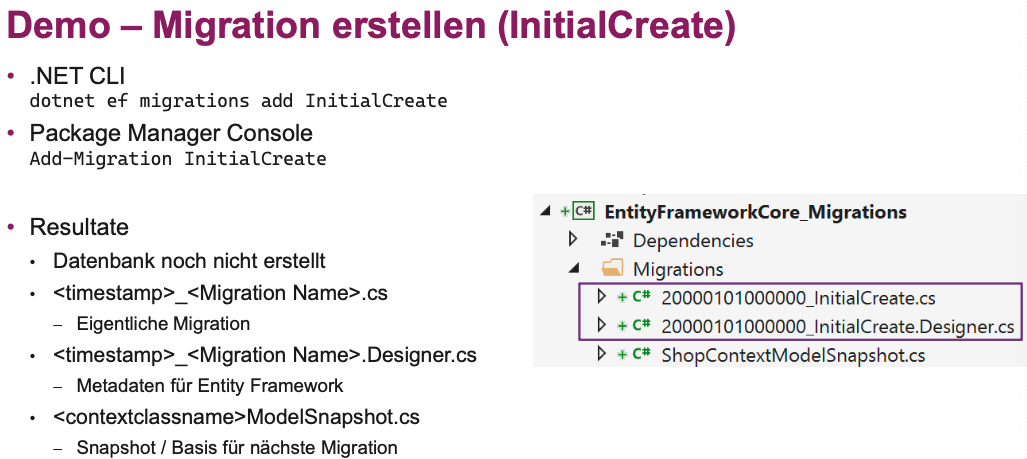
\includegraphics[width=.9\columnwidth]{dbmig1}\\
\vspace{2mm}
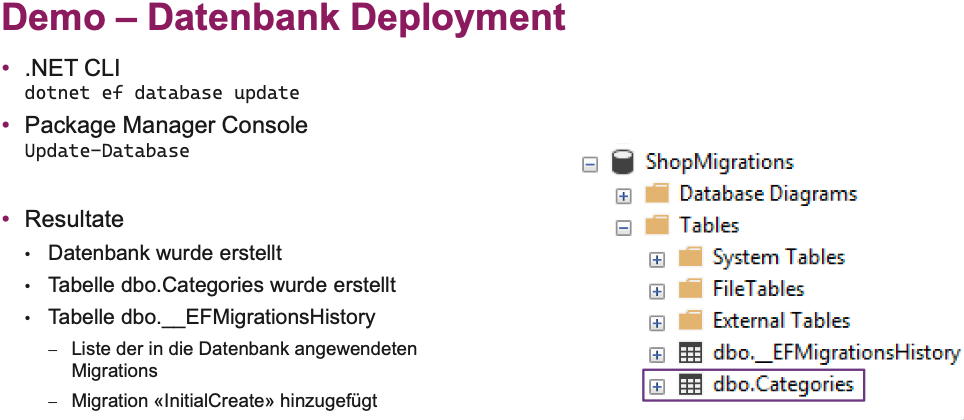
\includegraphics[width=.9\columnwidth]{dbmig2}\\
\vspace{2mm}
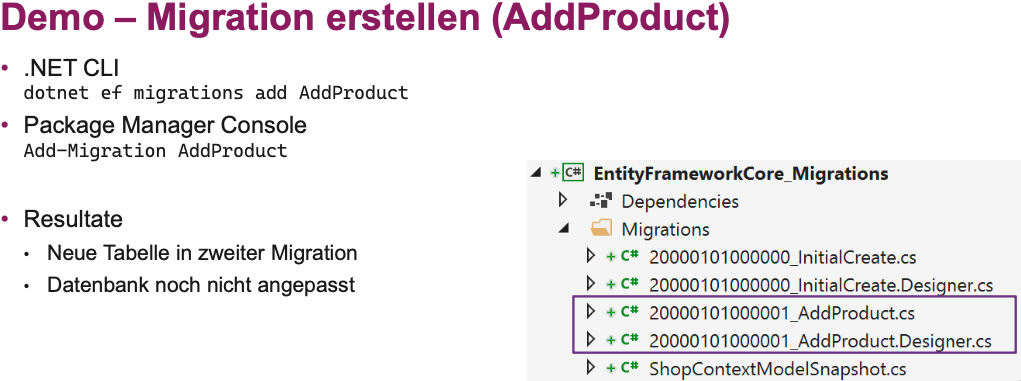
\includegraphics[width=.9\columnwidth]{dbmig3}\\
\vspace{2mm}
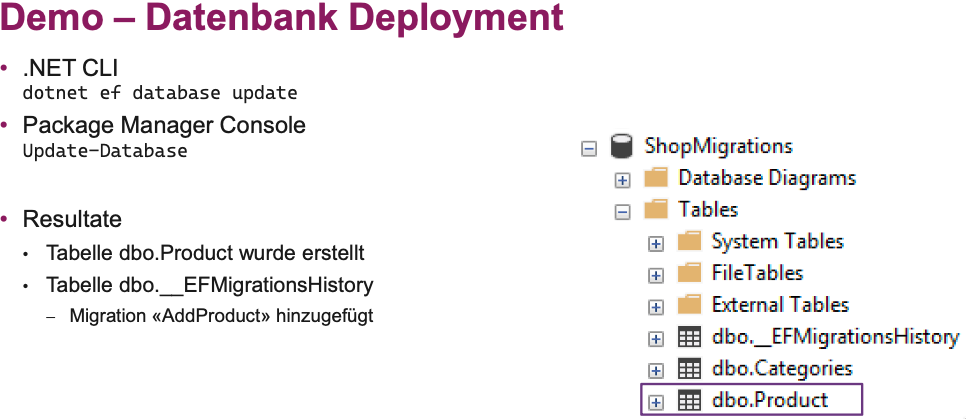
\includegraphics[width=.9\columnwidth]{dbmig4}\\
\subsubsection{Command CLI}
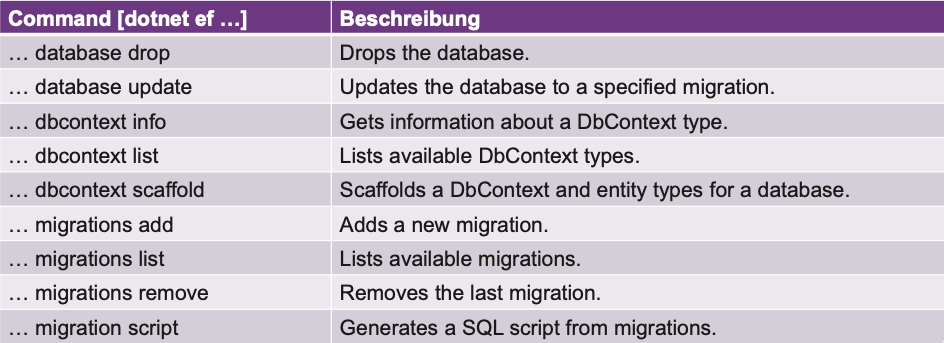
\includegraphics[width=.9\columnwidth]{commands}
\nfat{C\# API}
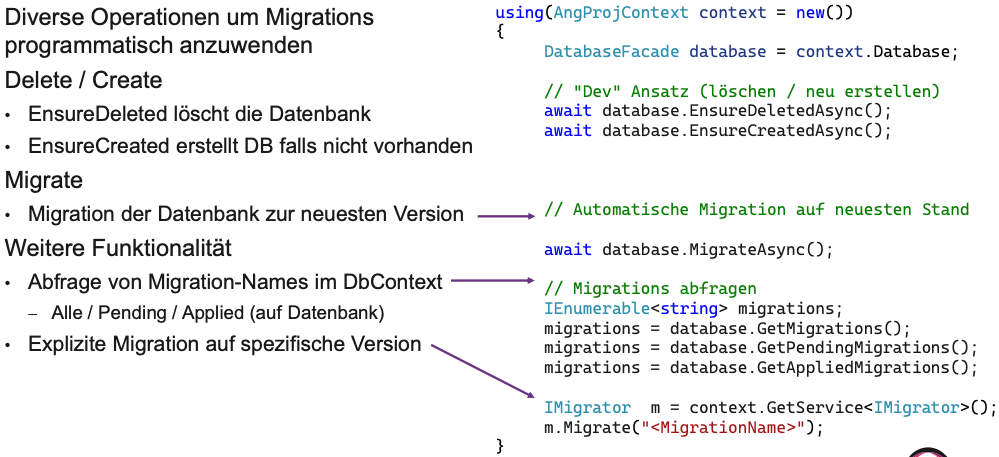
\includegraphics[width=\columnwidth]{migapi}
\end{multicols*}